%!TEX root=../main.tex


\section {The Zeeguu Platform}

A prototype of a learning ecosystem as described in the previous section is currently being bootstrapped at the Universities of Bern and Groningen. It is growing around an open platform dubbed Zeeguu. 

Figure \ref{fig:architecture} presents a very simplified version of the Zeeguu platform and ecosystem although it should be noted that the diagram is general enough for representing any learning ecosystem. The main components of the architecture in the case of Zeeguu are:

\begin{figure}[h!]
	% \centering
	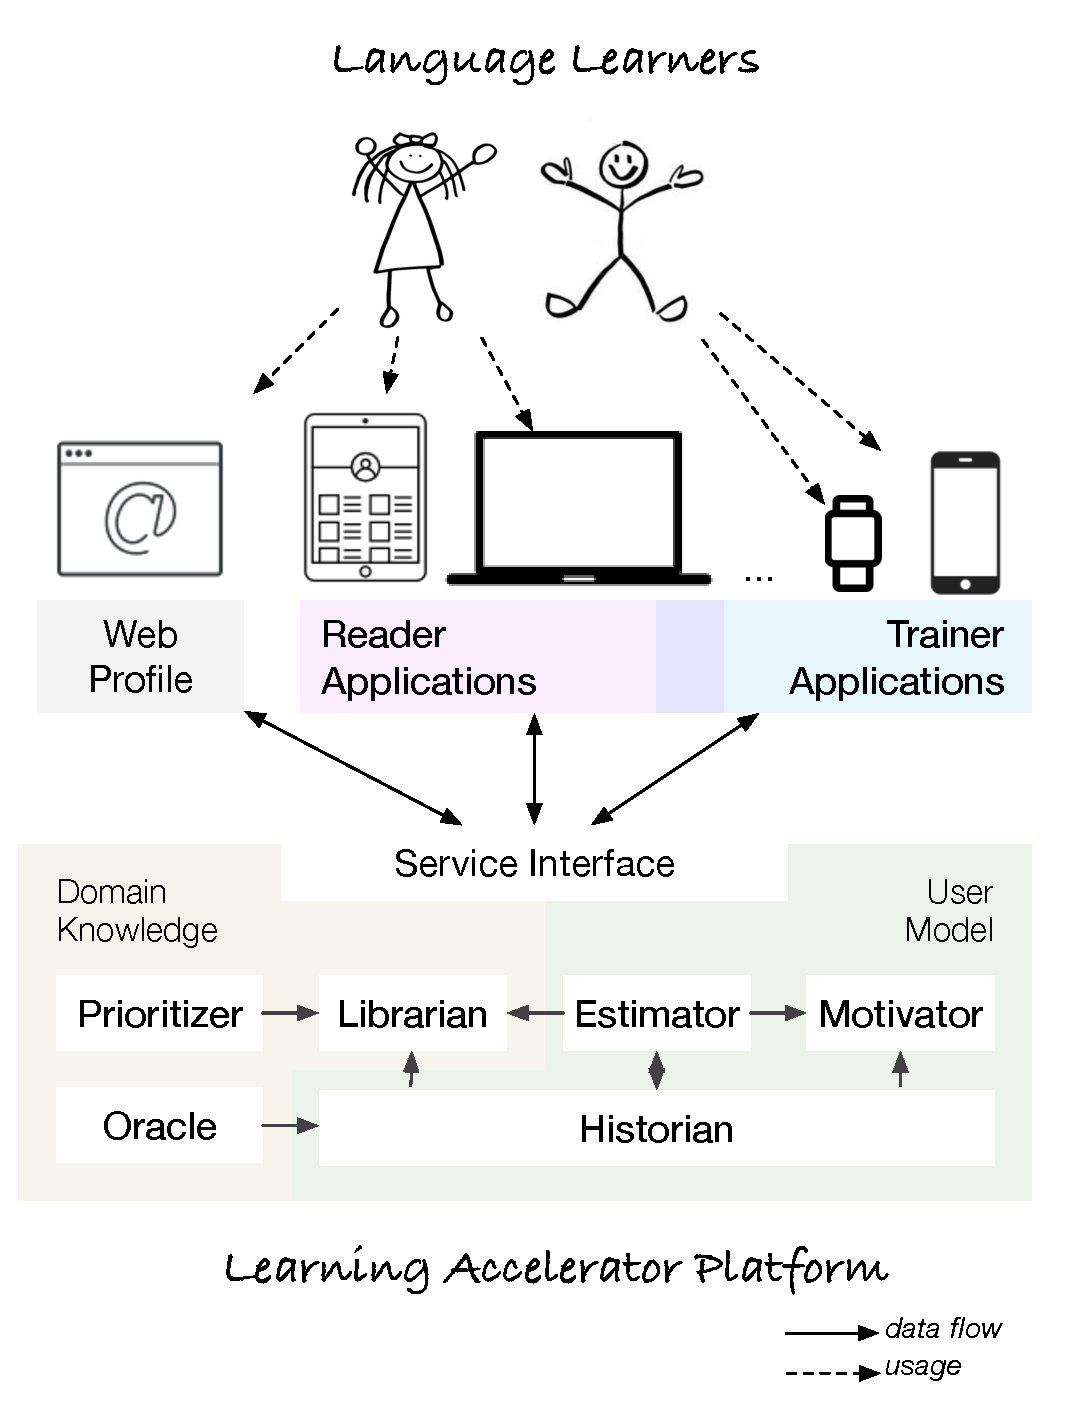
\includegraphics[width=\linewidth]{images/zeeguu-architecture.pdf}
	\caption{A very high-level view of the architecture of the Zeeguu ecosystem}
	\ml{to rename the things here to Reader / Trainer - Applications. }

	\label{fig:architecture}
\end{figure}


\begin{itemize}
	
	\item {\bf Reader Assistants} 
	support reading any kinds of materials in foreign languages. The reader applications must have two properties in common: 
		1) they should make it very convenient for the user to obtain translations for the texts he encounters in the foreign language. 
		2) they should track every event that provides a hint to the current user knowledge. In particular, every word that is being translated by the user indicates his lack of knowledge with respect to that particular word, and every word that is not being translate by the user indicates their knowledge of that word. 
	
		\item {\bf User Model Store} 
		% User Model Database
		% User Model Registry
		% User Model Store
		% User Profile Repository -- this would be better since... 
		is a core component of the learning ecosystem since it stores and orchestrates the exchange of information about the current and historical knowledge of the user. It needs to have several components, including: 

		\begin{itemize}

			\item The {\bf Interaction Historian} represents a centralized data warehouse that stores all the interactions of a learner with texts in the foreign language that are mediated by the Reader applications.

			\item The {\bf Knowledge Estimator} tries to approximate the current knowledge of the user based on the interaction history, and the feedback received from the Trainer agents, and other types of information that are available about the user

			\item The {\bf Oracle} is an agent which decides what are the most important items to be studied next by the learner. 
			\ml{could be talking about -- items to be encountered... not studied. the way in which the items will then later be encountered depends on the }
			% We envision multiple oracle implementations competing with each other

		\end{itemize}


	\item {\bf Trainer Agents} support the learner in practicing the vocabulary and must interact with the user model. A trainer application can request from the user model store information on which words are to be learned by the learner. But a trainer application must also provide back to the central user model information about how well the learner behaves with respect to a given word, otherwise this information will be lost. 
	
	% Two types of trainer agents are: 
	% \begin{itemize}
	% 	\item Librarians --  can recommend articles to read, music to listen to, movies to watch, etc.
	% 	\item Coaches -- which provide exercises for learning 
	% \end{itemize}
	% - Librarians -- 
	% - Coaches -- which use exercises to help the learner rehearse 


	
\end{itemize}

Note that as the Figure \ref{fig:architecture} suggests, the Reader Assistants and Trainer Agents need not be disjoint applications, but one application could provide both.

It might appear intuitive for the reader that the more contexts in which the reader is supported by applications from the ecosystem, the better the knowledge model of that learner that can be built, and the better the user experience. Such a learning ecosystem can thus present a network effect where its value will increase more than linear with the number of applications that contribute to it.

% Somewhere, we still have to discuss the question of: 
% - How are we going to maintain this ecosystem? who will provide the data storage and translation facilities for the long run? 
% - What are the incentives for new players to join the ecosystem?
% - ... 


